\section{Imaging-Sonar Forward Model}
\label{sec:forward-model}

Understanding how FLS forms an image is essential to reconstructing geometry from it. Our forward model treats the sonar readings as a collection of narrow azimuthal beams, each composed of a dense vertical fan of rays. The renderer explicitly models how these rays interact with the seafloor, how their returns combine into range–azimuth bins, and how physical factors such as incidence, gain, and spreading determine pixel intensities. 

\subsection{Seafloor Representation}
\label{sec:seafloor_rep}

We represent the seafloor as a discretized height field which can either be a Cartesian grid, or radially aligned with the sonar's azimuth beams. We place the sonar at the origin of a right-handed sensor frame, looking down -X with +Y right and +Z up (see Fig.~\ref{fig:sonar_overview}). All distances are in meters, and angles are in radians.

As shown in Fig. \ref{fig:heightfield_sideview}, in the Cartesian representation each entry in the height field is a perpendicular displacement from the X-Y plane. When using the polar representation we instead use \textit{angular heights} measured in radians. Therefore, as the height at a given point is varied it remains on a spherical shell of constant radius.


\begin{figure}[t]
  \centering
  \begin{minipage}{\columnwidth}
    \centering
    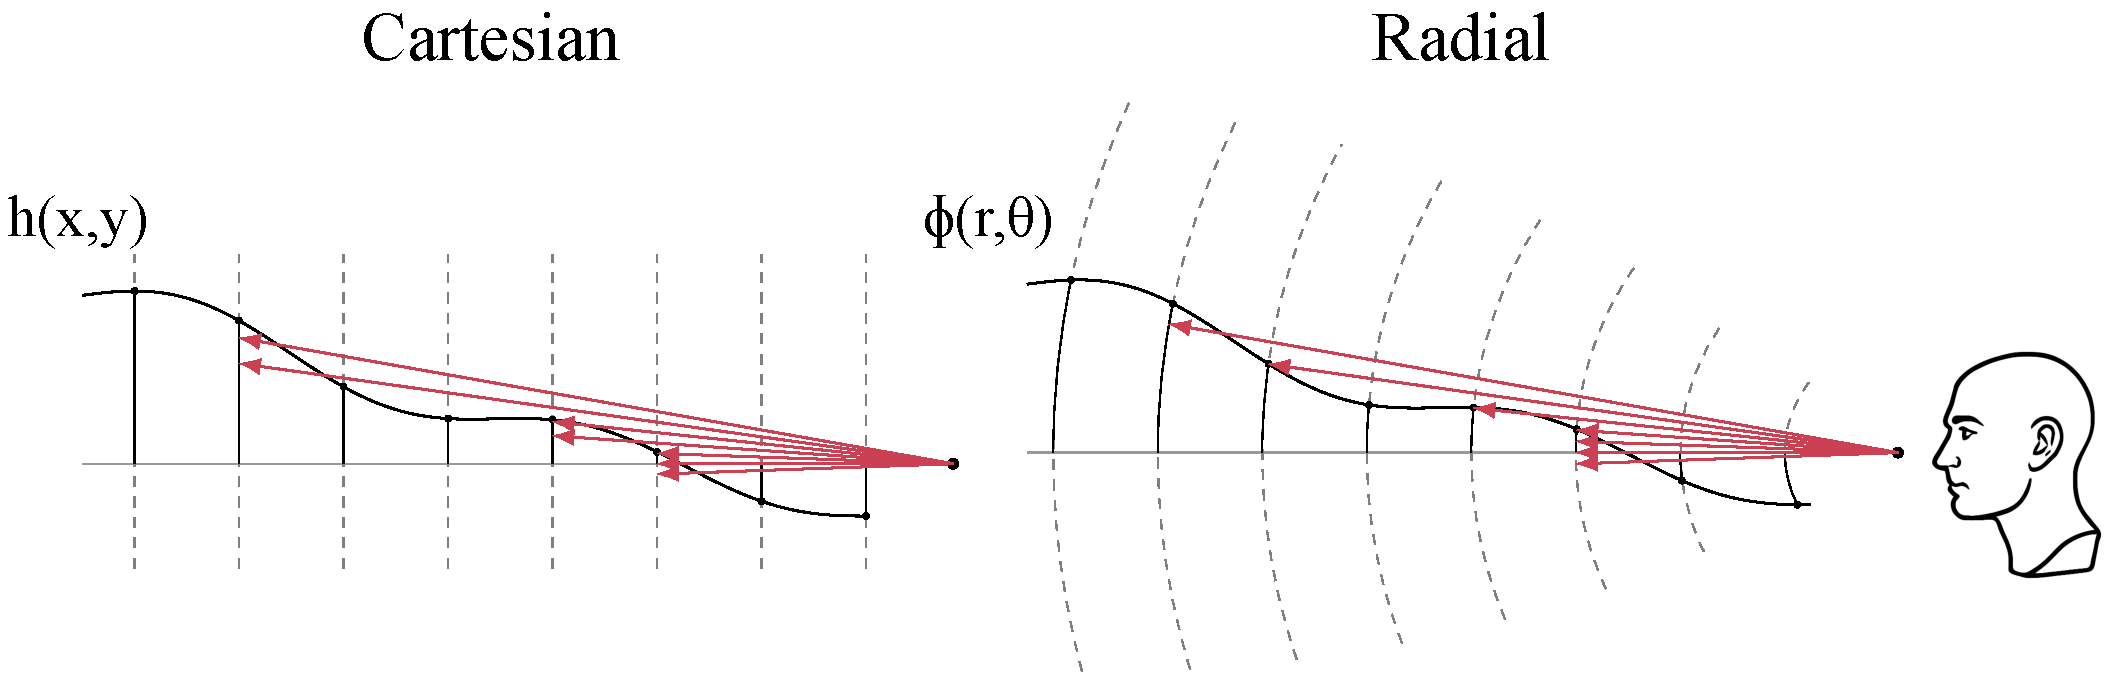
\includegraphics[width=1.0\columnwidth]{figs/cartesian_sideview.pdf}
    \caption{{\bf Side-view of the Cartesian (left) and polar (right) parameterizations} (\textit{cf.} Sec.~\ref{sec:seafloor_rep}). The polar height field stores angular heights, which vary along spherical shells of fixed radii. Ray intersections are determined by the first height entry which exceeds the height of the ray at that planar/spherical boundary.}
    \label{fig:heightfield_sideview}
  \end{minipage}
  
  \vspace{1em}
  
  \begin{minipage}{\columnwidth}
    \centering
    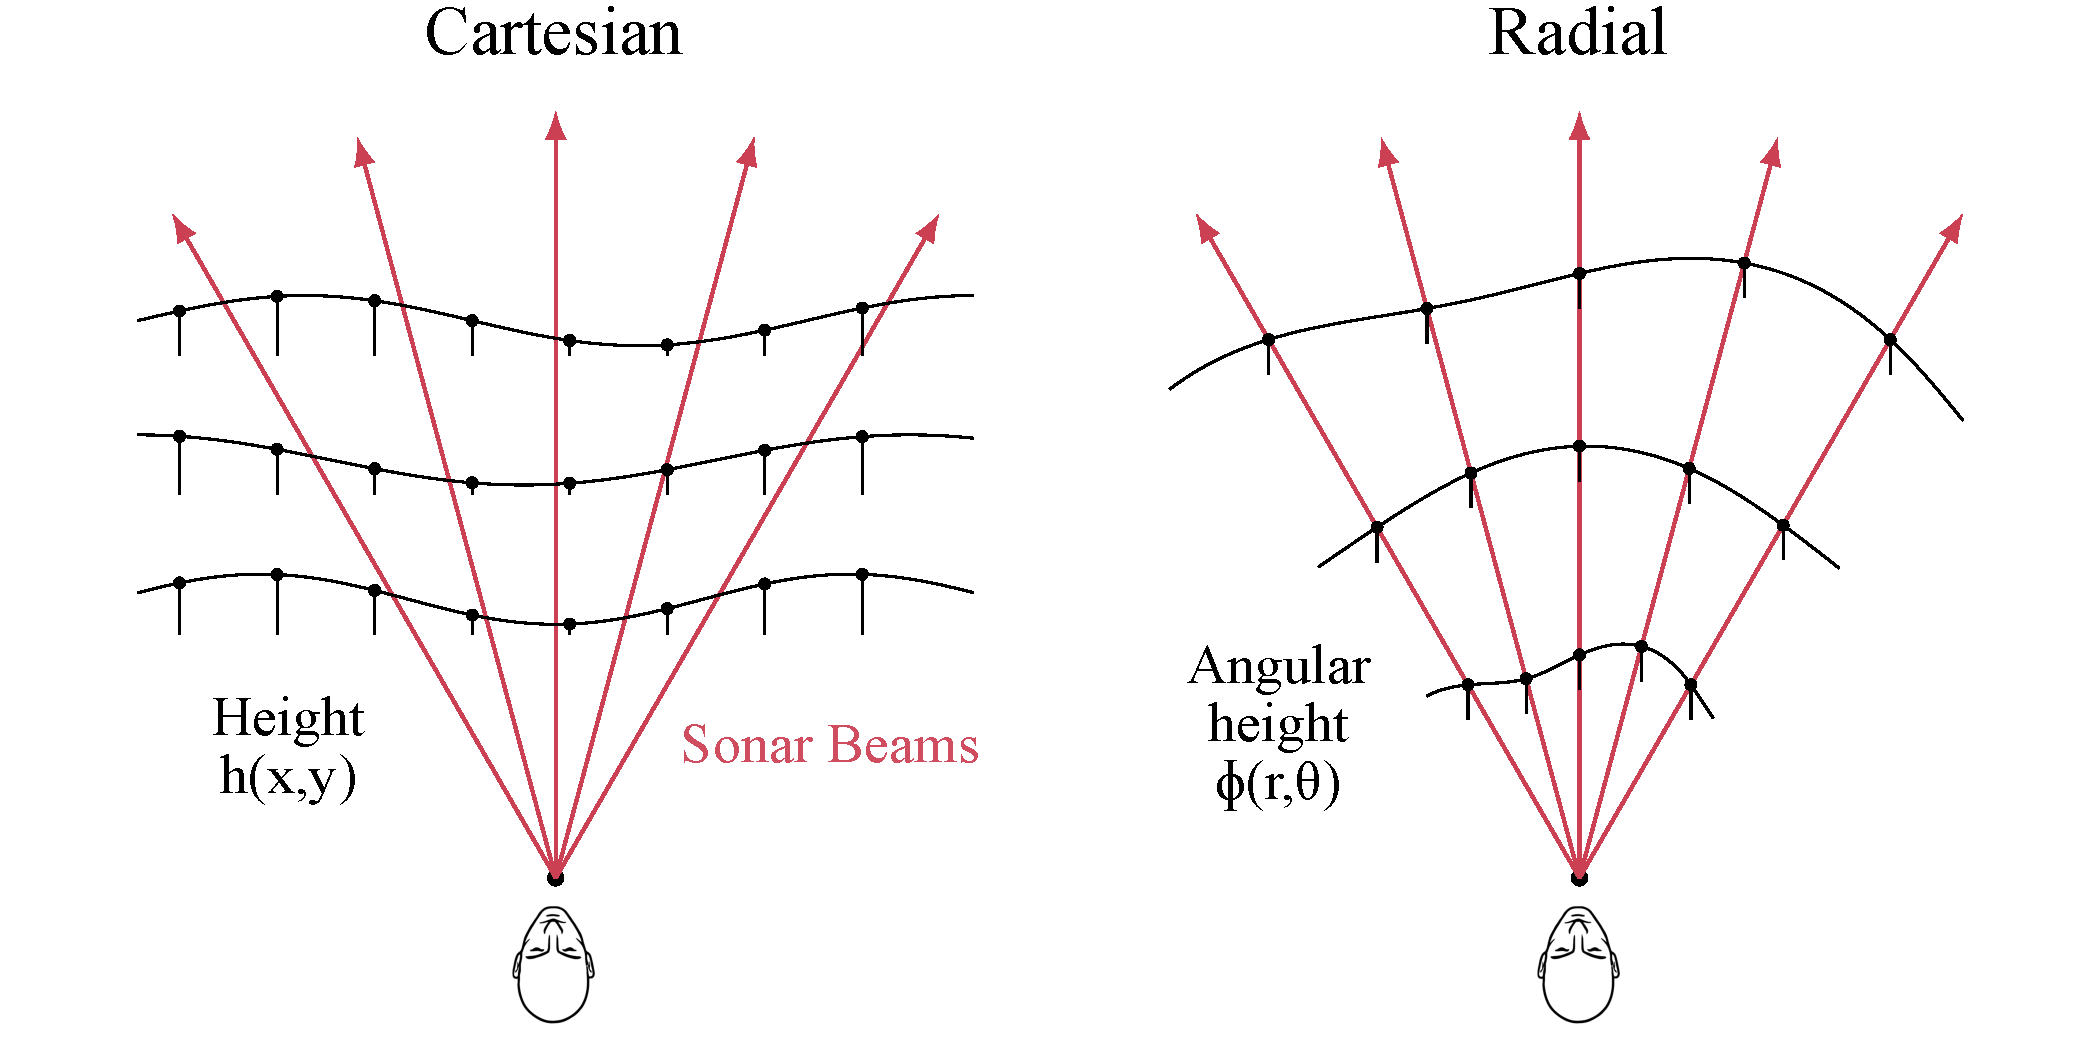
\includegraphics[width=1.0\columnwidth]{figs/cartesian_topview.pdf}
    \caption{{\bf Top-view of the Cartesian (left) and polar (right) parameterizations} (\textit{cf.} Sec.~\ref{sec:seafloor_rep}). The polar field is aligned to the FLS sampling grid.\vspace{-8mm}}
    \label{fig:heightfield_topview}
  \end{minipage}
  
  \vspace{1.5em}
  
\end{figure}

In Fig. \ref{fig:heightfield_topview} we demonstrate how the height field is aligned with the sensor beams in the polar setting. Each column in the 2D height field corresponds to an azimuthal angle, which is chosen to match the angles sampled by the sonar sensor. This formulation has the advantage of being more stable in the learning process, since changes in heights remain local in their effect on pixel brightnesses.
% In this representation, surface normals are obtained by differentiating the world-space surface position across the heightfield’s two local coordinates and taking their cross-product.

\subsection{Intersections and Reflectance}
\label{sec:reflectance}
We construct a dense ray fan for each beam sampled by the sonar. Given $n_\text{az}$ azimuth beams and $n_\text{el}$ elevation samples (default $n_\text{el}=6n_\text{bins}$), we uniformly sample $n_\text{el}$ rays along the vertical arclength of the sensor for each of the $n_\text{az}$ beams, for a total of $n_\text{az}\,n_\text{el}$ ray samples. In this way the beams are sampled at discrete angles, while the elevation sampling approximates a continuous fan.

In Cartesian representations, ray intersections can be estimated by interpolating heights at various ranges and comparing against ray heights at those locations. In the polar seafloor, intersections are even simpler. Since the ray travels along only a single column of the beam-aligned height field, intersections are determined by the first entry whose angular height exceeds the angular elevation component of the ray (see Fig.~\ref{fig:heightfield_sideview}). For inverse rendering these operations are made differentiable, as explained in Sec.~\ref{sec:differentiable_intersections}.

\looseness=-1
We model per-ray backscatter as a sum of diffuse and specular terms at the ray–surface intersection.
Let $\mathbf{n}_{r,\theta}$ denote the unit surface normal of the height field at \((r,\theta)\) and $\boldsymbol{\omega}_{\theta,\phi}$ the unit direction from the surface back to the sensor. 
Co-located FLS transmitter and receiver lets us parameterize reflectance by this single vector.
The diffuse factor is calculated as
\vspace{-1.5mm}
\begin{equation}
\mu = \mathrm{max}\:\!\big(0, \mathbf{n}_{r,\theta}\!\cdot\!\boldsymbol{\omega}_{\theta,\phi}\big),
\end{equation}
and the specular term is modeled as a reflection lobe,
\begin{equation}
\exp\left(-\frac{1-\boldsymbol{\omega}_\text{refl}\!\cdot\!\boldsymbol{\omega}_{\theta,\phi}}{\sigma_{\text{spec}}^2}\right), %= \exp\!\left(-\frac{1+\boldsymbol{\omega}_r\!\cdot\!\boldsymbol{\omega}_i}{\sigma_{\text{spec}}^2}\right),
\end{equation}
which takes maximum value when \(\boldsymbol{\omega}_{\theta,\phi}=\boldsymbol{\omega}_\text{refl}\), where \(\boldsymbol{\omega}_\text{refl}\) is the reflection direction given by
\begin{equation}
\boldsymbol{\omega}_\text{refl} = 2(\mathbf{n}\!\cdot\!\boldsymbol{\omega}_{\theta,\phi})\,\mathbf{n} - \boldsymbol{\omega}_{\theta,\phi}.
\end{equation}
The final reflectivity is then
\begin{equation}
f(r, \theta, \phi) = 
\Big[
\mu^{\gamma}
\;+\;
\exp\!\Big(-\frac{1-\boldsymbol{\omega}_\text{refl}\!\cdot\!\boldsymbol{\omega}_{\theta,\phi}}{\sigma_{spec}^2}\Big)
\Big]\,J,
\label{eq:reflectance}
\end{equation}
where $\gamma$ controls the diffuse falloff ($\gamma{=}1$ is Lambertian) and $\sigma_{spec}$ sets the specular lobe width. A geometric correction factor accounts for range spreading and foreshortening at range \(r\) as:
\vspace{-2mm}
\begin{equation}
J = \frac{r^2}{\max(\mu,\varepsilon)},
\end{equation}
with a small $\varepsilon$ for numerical stability.

\subsection{Image Formation and Processing}
From per-ray hit ranges (\(r\)) and reflectivities, intensities are spread into image bins. Gaussian binning weights are calculated as
\vspace{-1mm}
\[
\omega_k(r)\propto \exp\!\left[-\frac{1}{2}\left(\frac{u(r)-k}{\sigma_{\text{bins}}}\right)^{\!2}\right],
\]
where $u(r)$ is the fractional bin coordinate and $\sigma_{\text{bins}}$ controls spread. We apply a \(1/r^4\) correction factor to the reflectivities based on range \(r\) to account for two-way spherical geometric spreading, but implement a differentiable time-varying gain correction which optionally undoes this attenuation, as is commonly implemented in sonar sensor processing~\cite{Maclennan1986TVG}. Summed intensities are converted to log-amplitudes (dB) using $10\log_{10}(\cdot)$ compression.